% !TEX root = ../main.tex

\section{Introductory Remarks}

For better or worst, blockchain technologies like Ethereum have dramatically lowered the barrier to entry for developing and deploying financial technology. New tokens have been launched with a few clicks of a user interface, and large investment infrastructures have been developed and deployed with little regulatory oversight. Blockchain exchange services allow order-based trading of digital currencies, tokens, and other digital assets. Such exchanges are a key component to blockchain-based economic activity. 

For years, exchanges have operated either entirely off-chain by trusted operators or partially on-chain by semi-trusted operators. A fully on-chain exchange is feasible but considered too slow, at least for a public blockchain like Ethereum. We believe it is a very good time to do a deep dive into understanding precisely \textit{how slow} for the following reasons: (1) public blockchains are becoming faster (both in theory and slowly in practice) and the efficiency of an on-chain exchange will increase in time, (2) demand for on-chain trading is exemplified by the recent popularity of dealer-based (or quote-based) trading like Uniswap and Curve Finance, and (3) stablecoins have become a popular and allow on-chain trading with pricing in USD (or other government currency).

\paragraph{Contributions.} We design and implement \cm, a fully on-chain call market in Solidity---a high-level programming language for Ethereum. We choose Ethereum as a `hostile' environment for an orderbook: Ethereum is public (strongest adversary) and slow (lower-bound benchmark) relative to more scalable blockchains, including the anticipated Ethereum 2.0. \cm is intended as a simple module that developers can modify as they choose. By adding \cm to an ERC20 (or similar) token contract, everything that is needed for buying/selling tokens is immediately available on chain without involving any third party exchanges. \cm is non-custodial, transparent, and mitigates front-running attacks that are generally possible on-chain.

While Solidity and EVM are like many common programming languages, they also have quirks that require experimentation to best optimize performance (\eg factoring in the gas costs of operations, gas refunds, limits to Solidity's object oriented design, clearing mappings). We test five priority queues---the core data structure of the call market---and various options for cleaning up our data once finished with it. The bottom line is that the current benchmark for a \cm-esque design is in the low hundreds of trade executions per block on Ethereum today. This positions \cm as a feasible design for certain types of markets today (low liquidity, small number of traders) but also as an early study on technology that is likely to improve vastly in the coming years. 

% = = = = = = = = = = = = = = = = = = = = = = = = = = = = = = = = = = = = = = = = = =
% = = = = = = = = = = = = = = = = = = = = = = = = = = = = = = = = = = = = = = = = = =
% = = = = = = = = = = = = = = = = = = = = = = = = = = = = = = = = = = = = = = = = = =

\section{Preliminaries}

\subsection{Market Structure}

\paragraph{Execution systems.} There are three main approaches to arranging a trade~\cite{Har03}. In a \emph{quote-driven} market, a dealer uses their own inventory to offer a price for buying or selling an asset. In a \emph{brokered exchange}, a broker finds a buyer and seller. In an \emph{order-driven} market, offers to buy (\emph{bids}) and sell (\emph{offers}/\emph{asks}) from many traders are placed as orders in an orderbook. Order-driven markets can be \emph{continuous}, with buyers/sellers at any time adding orders to the orderbook (\emph{makers}) or executing against an existing order (\emph{takers}); or they can be \emph{called}, where all traders submit orders within a window of time and orders are matched in a batch like an auction. 

\subsection{Decentralized Order Matching}

\paragraph{Central exchanges (CEX).} Traditional financial markets (\eg NYSE and NASDAQ) use order-matching systems to arrange trades. An exchange will list one or more assets (stocks, bonds, derivatives, or more exotic securities) to be traded with each given its own orderbook priced in a currency (\eg USD). Exchanges for blockchain-based assets (also called cryptoassets by enthusiasts) can operate the same way, using a centralized exchange (CEX) design where a firm operates the platform as a trusted third party in every aspect: custodianship over assets/currency being traded, exchanging assets fairly, and offering the best possible price execution. Security breaches and fraud (\eg MtGox~\cite{TheHisto45:online}, QuadrigaCX~\cite{SEBIOrde83:online}, and many others) in centralized exchanges have become a common source of lost funds for users, while accusations of unfair trade execution have been levelled but are difficult to prove. 

\paragraph{On-chain orderbooks.} For trades between two blockchain-based assets (\eg a digital asset priced with a cryptocurrency, stablecoin, or second digital asset), order matching can be performed `on-chain' by deploying the order-matching system either on a dedicated blockchain or inside a decentralized application (DApp; \textit{a.k.a.} smart contract). In this model, traders entrust their assets to an autonomously operating DApp with known source code instead of a third party custodian that can abscond with or lose the funds. The trading rules will operate as coded, clearing and settling can be guaranteed, and order submission is handled by the blockchain---a reasonably fair and transparent system (but see front-running below). Finally, anyone can create an on-chain orderbook for any asset (on the same chain) at any time. While they sound ideal, performance is a substantial issue and the main subject of this paper. 

In this paper, we focus on benchmarking an orderbook for a public blockchain (\eg Ethereum). Ethereum is widely-used and we stand to learn the most from working in a performance-hostile environment (\ie Ethereum is good lower-bound). Exchanges could be given their own dedicated blockchain, where trade execution logic can be moved at the consensus level. Permissioned blockchains (\eg NASDAQ Linq, tZero) can also increase execution time and throughput, possibly with some reduction in transparency and trust.

\paragraph{On-chain dealers.} Another on-chain advantage is that other smart contracts, not just human users, can initiate trades, enabling broader decentralized finance (DeFi) applications. This has fuelled a resurgence in on-chain exchange but through a quote-driven design rather than an order-driven one. Automated market makers  (\eg Uniswap) have all the trust advantages of an on-chain orderbook, plus they are very efficient relative to an on-chain orderbook. The trade-off is that they operate as a dealer---the DApp exchanges assets from its own inventory. This inventory is loaded into the DApp by an investor who will not make money on the trades themselves, but hope for long term profit through trading fees. By contrast, an orderbook requires no upfront inventory and does not have to charge trading fees (but can). Finally, there is a complicated difference in their price dynamics (\eg market impact of a trade, slippage between the best bid/offer and actual average execution price, \etc)---deserving of an entire research paper to precisely define. We leave it as an assertion that with equal liquidity, orderbooks have more favourable price dynamics for traders.

\paragraph{Hybrid designs.} Before on-chain dealers became prominent in the late 2010s, the most popular design was hybrid order-driven exchanges with some trusted off-chain components and some on-chain functionality. Some (\eg EtherDelta) were envisioned as operating fully on-chain, but performance limitations drove developers to move key components, such as the order matching system, off-chain to a centralized database. A landscape of DEX designs exist: many avoiding taking custodianship of assets off-chain, and virtually all (for order-driven markets) operate the orderbook itself off-chain. A non-custodial DEX solves the big issue of a CEX---the operator stealing the funds---however trade execution is still not provably fair. A mitigation is to issue a proof of correct execution to the DApp (\eg Loopring) but these proofs have blindspots (discussed in section~\ref{sec:rollups}). \cm offers key advantages in this model. 

\subsection{Related Work}

\paragraph{Blockchain limitations and solution.} While an orderbook is a ledger and blockchains provide a distributed ledger, it is not straightforward to drop a continuous-time orderbook onto a blockchain. An older 2014 paper~\cite{clark2014decentralizing} on the `Princeton prediction market'~\cite{Bra13} motivates our work. The authors observe the following limitations of on-chain continous orderbooks: block intervals are slow and not continuous, there is no support for accurate time-stamping, transactions can be dropped or reordered by miners, fast traders can react to submitted orders/cancelations when broadcast to network but not in a block and have their orders appear first (as examined in later work on front-running: \cite{eskandari2019sok,daian2019flash}).

\paragraph{Call markets.} The researchers propose using a call market instead of a continuous-time market~\cite{clark2014decentralizing}. Orders are collected and placed into the orderbook over a window of time (\eg 1 or more blocks), then the market is closed and the orders are processed in batch: the best bids are matched to the best asks in order. If the prices overlap, the miner keeps the difference (which they could extract anyways through front-running). Call markets largely side-step front-running attacks from other traders because reordering trades has no impact (discussed more in section~\ref{sec:front}). The paper does not include an implementation and was envisioned as an alt-coin (Ethereum was still in development in 2014) with market closing being done by the miners themselves as part of the blockchain logic.

Large exchanges, like the NYSE and NASDAQ, use a two minute call market every day at opening and closing time (in between, the exchange runs as a continuous time market). Other exchanges, called crossing networks, also operate as a call market at various times throughout the trading day.\footnote{A crossing network uses a secondary market for determining the closing price. Many prominent crossing networks are operated internally within a brokerage for its clients, and often as a `	dark pool' with an unpublished orderbook.} Call market are studied widely in finance~\cite{Har03}. Time-sensitive traders submit orders early, especially in crossing networks that close at a randomly determined time (traders risk missing the call if they wait too long). A blockchain happens to provide this function naturally, as blocks are published unpredictably. Price-sensitive traders wait to base their pricing off the already submitted orders and do not mind missing a call if it obtains them a better price. 


\paragraph{Other Literature.}
% Madiba -> pulp.bib
% Velocity, 
% FuturesMex~\cite{massacci2018futuresmex}
% Findel 
% Libra~\cite{mavroudis2019libra}
% Arwen
% Tesseract (SGX-exchange)~\cite{bentov2017tesseract}
% Christopher Thorpe

% = = = = = = = = = = = = = = = = = = = = = = = = = = = = = = = = = = = = = = = = = =
% = = = = = = = = = = = = = = = = = = = = = = = = = = = = = = = = = = = = = = = = = =
% = = = = = = = = = = = = = = = = = = = = = = = = = = = = = = = = = = = = = = = = = =

\section{Priority Queues}\label{sec:pq}

% = = = = = = = = = = = =Operations for a generic Priority Queue Table = = =  = = = = = = = = = = = %
\begin{table}[t]
\setlength{\tabcolsep}{0.01\tabcolsep}% Shrink \tabcolsep
\centering
\begin{tabular}{|c|c|}
\hline

\textbf{Operation}   & \textbf{Description}    \\ \hline

% = = = = = = = = = = = = = = = = = = = = = = = = = = = = = = = = = = = = = = = = = = = = = = = = %
	\textbf{Enqueue()}       	& Inserts an element into the priority queue                        \\ \hline
	\textbf{Dequeue()}		& Removes and returns the highest priority element 		\\ \hline
	\textbf{isEmpty()}			& Checks if the priority queue is empty 					\\ \hline
% = = = = = = = = = = = = = = = = = = = = = = = = = = = = = = = = = = = = = = = = = = = = = = = =  %

\end{tabular}
\caption{\footnotesize{Operations for a generic priority queue.}
\label{tab:PQ_API}}
\end{table}
% = = = = = = = = = = = = = = = = = = = = =  = = = = = = = = = = =  = = = = = = = = = == = = =  = =%

In designing \cm within Ethereum's gas model, performance is the main bottleneck. For a call market, processing all the trades and closing the market is the most time consuming step. The most critical design decision is the data structure for holding orders. While data structures are well studied for many languages, Solidity/EVM has its own unique aspects (\eg gas refunds, a relatively cheap mapping data structure, only partial support for object oriented programming) that creates difficulties in assessing which will perform best without actually deploying and evaluating each variant. 

When closing a call market, the orders are examined in order: highest to lowest price for bids, and lowest to highest price for asks. It most circumstances, the market closing algorithm does not have to consider any deeper bids/asks from the list when choosing whether the current best bid and ask can be fulfilled. The only exceptions are in the case of a tie on price or a canceled order, both of which we return to later. For this reason, the ideal data structure for storing bids/asks is a \textit{priority queue} (see Table~\ref{tab:PQ_API}) where each order's priority is its price. Specifically, we use two PQs---one for bids where the highest price is the highest priority, and one for asks where the lowest price is the highest priority. 

There are numerous ways of implementing a PQ. A PQ has an underlying list---common options include a static array, dynamic array, and linked list. The most expensive operation is keeping the data sorted---common options include (i) sorting during each enqueue, (ii) sorting for each dequeue, or (iii) splitting the difference by using a heap as the underlying data structure. Respectively, the time complexities are (i) linear enqueue and constant dequeue, (ii) constant enqueue and linear dequeue, and (iii) logarithmic enqueue and logarithmic dequeue. As closing the market is very expensive with any PQ, we rule out using (ii) as fully sorting while dequeuing would be prohibitive. We experiment with the following 5 options for (i) and (iii):

\begin{enumerate}

\item \textbf{Heap with Dynamic Array.} A heap is a type of binary tree data structure that comes in two forms of a (i) Max-Heap and (ii) Min-Heap. All the nodes of tree are in a specific order and the root of the tree always represents the highest priority item of the data structure (the largest and smallest values in the Max-Heap and Min-Heap respectively). We implemented a priority queue with a heap that stores its data in a dynamically-sized array. 

\item \textbf{Heap with Static Array.} A heap can be also represented by a Solidity storage array in which the storage is statically allocated. To do this, we pass the required size of the array as a constructor parameter to the priority queue smart contract. 

\item \textbf{Heap with Mapping.} In the above implementations, the heap stores the entire order (as a struct) in the heap. In this variant, we store the order struct in a Solidity mapping and store the mapping's key in the heap.  

\item \textbf{Linked List.} In this variant, we insert a new element into its correct position (based on its price) when running enqueue. The PQ itself stores elements in a linked list (enabling us to efficiently insert a new element between two existing elements). Solidity is described as object-oriented but the equivalent of an object is an entire smart contract. Therefore an object-oriented linked list must either (i) create each node in the list as a struct---but this is not possible as Solidity does not support recursive structs---or (ii) make every node in the list its own contract. The latter option seems wasteful and unusual, but we try it out anyways. Thus each node is its own contract and contains the order data and a pointer to the address of the next contract in the list.

\item \textbf{Linked List with Mapping.} Finally, we try a variant of a linked list using a Solidity mapping. The value of the mapping is a struct with order data and the key of the next (and previous) node in the list. The contract stores the key of the first node (head) in the list. 

\end{enumerate}

% = = = = = = = = = = = = = = = = = = = = = = = = = = = = = = = = = = = = = = = = = =

\subsection{Priority Queue Evaluation} 

\subsubsection{Enqueue performance.} We implemented, deployed, and tested each priority queue using Truffle and Ganache.\footnote{Github: Link removed for anonymity.} We tried a variety of tests (including testing the full call market with each varient) with consistent results in performance. A simple test to showcase the performance profile is shown in Figure~\ref{fig:random_insertion}. We simply enqueue 50 integers chosen at random from a fixed interval in each PQ variant. The bigger the PQ gets, the longer enqueue takes---a linear increase for the linked list variants, and logarithmic for the heap variants. 

% = = = = = = = = = = = = = = = = = = = = = = = = = = = = = = = = = = = = = = = =  %

\begin{figure}[t]
\centering
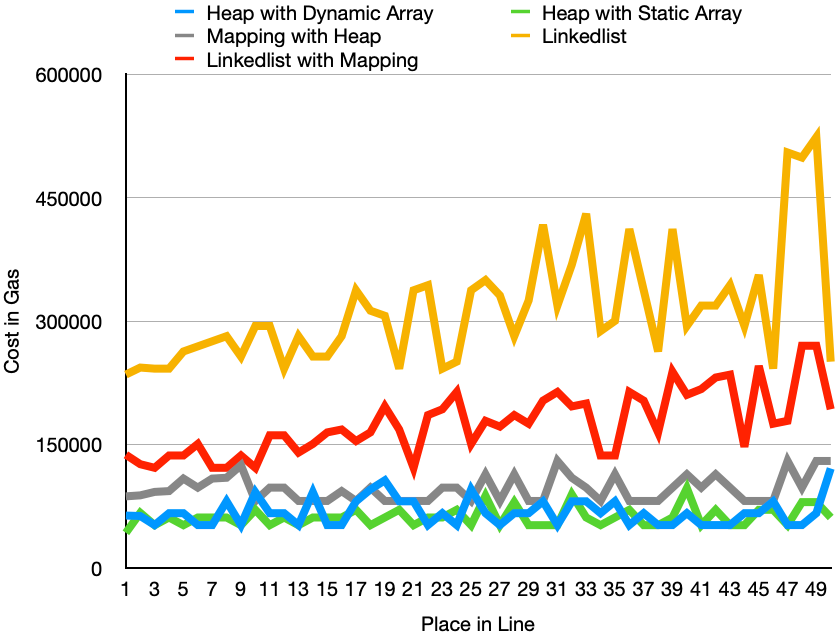
\includegraphics[width=0.8\textwidth]{fig/random_insertion.png}
\caption{\footnotesize{Gas costs for enqueuing random items into five different priority queue variants. For the x-axis, a value of 10 indicates it is the 10th number entered in the priority queue. The y-axis is the cost of enqueue in gas.}  \label{fig:random_insertion}}
\end{figure}

% = = = = = = = = = = = = = = = = = = = = = = = = = = = = = = = = = = = = = = = =  %

% !TEX root = ../main.tex

% = = = = = = = = = = = =Gas costs and refunds for Dequeueing 50 integers from each PQ  = = = = = = = = = = = = =  %

\begin{table}[t]
\setlength{\tabcolsep}{0.2\tabcolsep}% Shrink \tabcolsep
\centering
\begin{tabular}{|c|c|c|l|}

\multicolumn{1}{c}{} & \headrow{\footnotesize Gas Costs (\texttt{gasUsed})} & \headrow{\footnotesize Refund (Manual)} & \headrow{\footnotesize Full Refund?} \\ \hline

% = = = = = = = = = = = = = = = = = = = = = = = = = = = = = = = = = = = = = = = = = = = = = = = = = = = = = = = = = = = = = = = = = = = = = = %
Heap with Dynamic Array       	& 2,518,131          & 750,000     &\full                  \\ \hline
% = = = = = = = = = = = = = = = = = = = = = = = = = = = = = = = = = = = = = = = = = = = = = = = = = = = = = = = = = = = = = = = = = = = = = = %
Heap with Static Array          	& 1,385,307                             & 750,000      &\full                \\ \hline
% = = = = = = = = = = = = = = = = = = = = = = = = = = = = = = = = = = = = = = = = = = = = = = = = = = = = = = = = = = = = = = = = = = = = = = %
Heap with Mapping 			& 2,781,684                            & 1,500,000    &\full                 \\ \hline
% = = = = = = = = = = = = = = = = = = = = = = = = = = = = = = = = = = = = = = = = = = = = = = = = = = = = = = = = = = = = = = = = = = = = = = %
Linked List                     		& 557,085               	           & 1,200,000      &\full                \\ \hline
% = = = = = = = = = = = = = = = = = = = = = = = = = = = = = = = = = = = = = = = = = = = = = = = = = = = = = = = = = = = = = = = = = = = = = = %
Linked List with Mapping      	& 731,514              	     	  &  3,765,000      &\full                 \\ \hline
% = = = = = = = = = = = = = = = = = = = = = = = = = = = = = = = = = = = = = = = = = = = = = = = = = = = = = = = = = = = = = = = = = = = = = = %

\end{tabular}
\caption{The gas metrics associated with dequeuing 50 integers from five priority queue variants. For the refund, (\full) indicates the  refund was capped at the maximum amount and (\prt) means a greater refund would be possible.
\label{tab:PQUnitTests}}
\end{table}
% = = = = = = = = = = = = = = = = = = = = = = = = = = = = = = = = = = = = =  %


% = = = = = = = = = = = = = = = = = = = = = = = = = = = = = = = = = = = = = = = =  %
%  = = = = = = Table 2 (dequeue) Conversions = = = = = = %
%
%As of July 2020,  $1 gas = 56\times10^{-9} ether$\footnote{https://ethstats.net/} and 1 ether = \$238.33\footnote{https://coinmarketcap.com/}.
%
%$Transaction cost (eth) = GasUsed (unit) \times Gas Price (eth)$ 
%
%%  = = = = = = Transaction Costs in eth = = = = = = %
%
%Heap with Dynamic Array:    		$2,518,131 \times 56\times10^{-9} = 141,015,336\times 10^{-9}$
%Heap with Dynamic Array:     		$1,385,307 \times 56\times10^{-9} = 77,577,192\times 10^{-9}$
%Heap with Mapping:              		$2,781,684 \times 56\times10^{-9} = 155,774,304\times 10^{-9}$
%Linked List:						$557,085 \times 56\times10^{-9} = 	31,196,760\times 10^{-9}$
%Linked List with Mapping:			$731,514 \times 56\times10^{-9} = 	40,964,784\times 10^{-9}$
%
%%  = = = = = = Transaction Costs in USD = = = = = = %
%
%Heap with Dynamic Array:    		$141,015,336\times 10^{-9} \times 238.33 = \$33.60$
%Heap with Dynamic Array:     		$77,577,192\times 10^{-9} \times 238.33 = \$18.48$
%Heap with Mapping:              		$155,774,304\times 10^{-9} \times 238.33 = \$37.12$
%Linked List:						$31,196,760\times 10^{-9} \times 238.33 = \$7.43$
%Linked List with Mapping:			$40,964,784\times 10^{-9} \times 238.33 = \$9.76$
%
% = = = = = = = = = = = = = = = = = = = = = = = = = = = = = = = = = = = = =  %


% = = = = = = = = = = = = = = = = = = = = = = = = = = = = = = = = = = = = = = = =  %


\subsubsection{Dequeue performance.} For each PQ variant storing 50 random integers, the \texttt{Dequeue()} function is iterated until the data structure is empty. The total gas cost for fully dequeuing the priority queue variants is outlined in Table~\ref{tab:PQUnitTests}. These tests are performed using the following Ethereum gas metrics: block gas limit $=$11,741,495 and 1 gas $=$ 56 gwei.\footnote{EthStats (July 2020): \url{https://ethstats.net/}} Dequeuing removes data from the contract's storage. Recall this results in a gas refund. Based on our manual estimates (EVM does not expose the refund counter), every variant receives the maximum gas refund possible (\ie half the total cost of the transaction). In other words, each of them actually consumes twice the \texttt{gasUsed} amount in gas before the refund, however none of them are better or worst based on how much of a refund they generate.  

\subsubsection{Discussion.} Based on enqueuing, the heap variants are the cheapest in terms of gas, while based on dequeuing, the link list variants are cheapest. This is in accordance with the theoretical worst-case time complexity for each. However, (i) the linked list variants are materially cheaper than the heap variants at dequeuing, and (ii) dequeuing in a call market must be done as a batch, whereas enqueuing is paid for one at a time by the trader submitting the order, and (iii) Ethereum will not permit more than hundreds of orders so the asymptotic behaviour is not a significant factor. For these reasons, we suggest using a linked list variant for this specific application. As it can be seen in Figure~\ref{fig:random_insertion}, the associated cost for inserting elements into a linked list PQ is significantly greater than the linked list with mapping, as each insertion cause the creation of a new contracts. Accordingly, we choose to implement the call market with the linked list with mapping. Overall this PQ balances a moderate gas cost for insertion (\ie order submission) with one for removal (\ie matching the orders). 

% = = = = = = = = = = = = = = = = = = = = = = = = = = = = = = = = = = = = = = = =  %

\subsection{Cost/Benefit of cleaning up after yourself}
\label{sec:LLvsLLMapping}
\label{sec:gasrefund}

% !TEX root = ../main.tex


% = = = = = = = = = = = =Gas costs and refunds for Dequeueing 50 integers from each PQ  = = = = = = = = = = = = =  %

\begin{table}[t]
\centering
\begin{tabular}{|p{7cm}|r|r|r|}

\multicolumn{1}{c}{\.} & \headrow{Gas Costs (\texttt{gasUsed})} & \headrow{Refund (Manual)} & \headrow{Full Refund?} \\ \hline

% = = = = = = = = = = = = = = = = = = = = = = = = = = = = = = = = = = = = = = = = = = = = = = = = = = = = = = = = = = = = = = = = = = = = = = %
% = = = = = = = = = = = = = = = = = = = = = = = = = = = = = = = = = = = = = = = = = = = = = = = = = = = = = = = = = = = = = = = = = = = = = = %
Linked List w/o \texttt{SELFDESTRUCT}         		& 721,370          & 0     &$\times$  \\ \hline
Linked List with \texttt{SELFDESTRUCT}       		& 557,085          & 1,200,000     &\full  \\ \hline
Linked List with Mapping and w/o \texttt{DELETE}    & 334,689          & 765,000     &\full  \\ \hline
Linked List with Mapping and \texttt{DELETE}		& 731,514          & 3,765,000     &\full  \\ \hline

% = = = = = = = = = = = = = = = = = = = = = = = = = = = = = = = = = = = = = = = = = = = = = = = = = = = = = = = = = = = = = = = = = = = = = = %
% = = = = = = = = = = = = = = = = = = = = = = = = = = = = = = = = = = = = = = = = = = = = = = = = = = = = = = = = = = = = = = = = = = = = = = %
% = = = = = = = = = = = = = = = = = = = = = = = = = = = = = = = = = = = = = = = = = = = = = = = = = = = = = = = = = = = = = = = = = = = = = = %

\end{tabular}
\caption{The gas metrics associated with dequeuing 50 numbers from five priority queues variants. For the refund, (\full) indicates the  refund was capped at the maximum amount and \textblue{(\prt) means a greater refund would be possible}.\label{tab:cleaning}}
\end{table}


%  = = = = = = Table 3 (cleaning.tex) Conversions = = = = = = %

%As of July 2020,  $1 gas = 56\times10^{-9} ether$\footnote{https://ethstats.net/} and 1 ether = \$238.33\footnote{https://coinmarketcap.com/}.
%
%$Transaction cost (eth) = GasUsed (unit) \times Gas Price (eth)$ 
%
%%  = = = = = = Transaction Costs in eth = = = = = = %
%
%Linked List with \texttt{SELFDESTRUCT}:     				$557,085 \times 56\times10^{-9} =  31,196,760\times 10^{-9}$  
%Linked List w/o \texttt{SELFDESTRUCT}:     				$721,370 \times 56\times10^{-9} =  40,396,720\times 10^{-9}$ 
%Linked List with Mapping and \texttt{DELETE}:    			$731,514 \times 56\times10^{-9} =  40,964,784\times 10^{-9}$ 
%Linked List with Mapping and w/o \texttt{DELETE}: 		$334,689 \times 56\times10^{-9} =  18,742,584\times 10^{-9}$ 
%
%%  = = = = = = Transaction Costs in USD = = = = = = %
%
%Linked List with \texttt{SELFDESTRUCT}:     				$31,196,760\times 10^{-9}  \times 238.33 = \$7.43$
%Linked List w/o \texttt{SELFDESTRUCT}:     				$40,396,720\times 10^{-9} \times 238.33 = \$9.62$
%Linked List with Mapping and \texttt{DELETE}:    			$40,964,784\times 10^{-9}  \times 238.33 = \$9.76$
%Linked List with Mapping and w/o \texttt{DELETE}: 		$18,742,584\times 10^{-9} \times 238.33 = \$4.46$
% = = = = = = = = = = = = = = = = = = = = = = = = = = = = = = = = = = = = =  %



One consequence of a linked list is that a new contract is created for every node in the list. Beyond being expensive for adding new nodes (a cost that will be bared by the trader in a call market), it also leaves a large footprint on the Ethereum blockchain, especially if we leave the nodes on the blockchain in perpetuity (\ie we just update the head node of the list and leave the previous head `dangling.'). However in a PQ, nodes are only removed from the head of the list; thus the node contracts could be `destroyed' one by one using an extra operation, \texttt{SELFDESTRUCT}, in the \texttt{dequeue()} function. As shown in Table~\ref{tab:cleaning}, the refund from doing this outweighs to the cost of the extra computation: gas costs are reduced from 721K to 557K.  This suggests a general principle: cleaning up after yourself will pay for itself in gas refunds. Unfortunately, this is not universally true as shown by applying the same principle to the Linked List with Mapping. 

Dequeuing in a linked list with mapping can be implemented in two ways. The simplest approach is process a node, update the head pointer, and leave the `removed' node's data behind in the mapping untouched (where it will never be referenced again). Alternatively we can call \texttt{DELETE} on each mapping entry once we are done with a node in the PQ. Deleting a storage variable is identical to setting a non-zero variable to zero (\texttt{SSTORE} 0) that costs 20,000 gas but with 15,000 refunded---a net positive gas cost~\cite{wood2014ethereum}. As it can be seen in the last two rows of Table~\ref{tab:cleaning}, leaving the data on chain is cheaper then cleaning it up.

The lesson here is that gas refunds incentivize developers to clean up storage variables they will not use again, but it is highly contextual as to whether it will pay for itself. Further the cap on the maximum refund means that refunds are not fully received for large cleanup operations (however removing the cap impacts the miners' incentives to include the transaction). This is a complicated and under-explored area of Ethereum in the research literature. For our own work, we strive to be good citizens of Ethereum and cleanup to the extent that we can---thus all PQs in Table~\ref{tab:PQUnitTests} implement some cleanup and we select Linked List with Mapping and \texttt{DELETE} for \cm.



% = = = = = = = = = = = = = = = = = = = = = = = = = = = = = = = = = = = = = = = = = =
% = = = = = = = = = = = = = = = = = = = = = = = = = = = = = = = = = = = = = = = = = =
% = = = = = = = = = = = = = = = = = = = = = = = = = = = = = = = = = = = = = = = = = =

\section{Call Market Design}

%GitHub repo:  \footnote{\CallMarketRepo}

% !TEX root = ../main.tex

% = = = = = = = = = = = = = = = = = = = = =Call market operations Table = = = = = = = = = = = =  = = = = = =  %
\begin{table}[t]
\begin{tabular}{|l|l|}
\hline
\multicolumn{1}{|c|}{\textbf{Operation}} & \multicolumn{1}{c|}{\textbf{Description}}                            			\\ \hline

% = = = = = = = = = = = = = = = = = = = = = = = = = = = = = = = = = = = = = = = = = = = = = = = = = = = =  %
	depositToken()                           & Deposits ERC20 standard compliant tokens in \cm smart contract \\ \hline
% = = = = = = = = = = = = = = = = = = = = = = = = = = = = = = = = = = = = = = = = = = = = = = = = = = = =  %
	depositEther()                           	& Deposits ETH in \cm smart contract                        			 \\ \hline
% = = = = = = = = = = = = = = = = = = = = = = = = = = = = = = = = = = = = = = = = = = = = = = = = = = = =  %
	openMarket()                             & Opens the market                                                    					 \\ \hline
% = = = = = = = = = = = = = = = = = = = = = = = = = = = = = = = = = = = = = = = = = = = = = = = = = = = =  %
	closeMarket()                            & Closes the market and processes the orders       \\ \hline
% = = = = = = = = = = = = = = = = = = = = = = = = = = = = = = = = = = = = = = = = = = = = = = = = = = = =  %
	submitBid()                              & Inserts the upcoming bid order messages inside the priority queue    \\ \hline
% = = = = = = = = = = = = = = = = = = = = = = = = = = = = = = = = = = = = = = = = = = = = = = = = = = = =  %
	submitAsk()                              & Inserts the upcoming ask order messages inside the priority queue    \\ \hline
% = = = = = = = = = = = = = = = = = = = = = = = = = = = = = = = = = = = = = = = = = = = = = = = = = = = =  %
	claimTokens()                           & Transfers tokens to the traders                       			\\ \hline
% = = = = = = = = = = = = = = = = = = = = = = = = = = = = = = = = = = = = = = = = = = = = = = = = = = = =  %
	claimEther()                             & Transfers ETH to the traders                       			\\ \hline
% = = = = = = = = = = = = = = = = = = = = = = = = = = = = = = = = = = = = = = = = = = = = = = = = = = = =  %
\end{tabular}
\caption{\footnotesize{Primary operations of \cm smart contract.}
\label{tab:cm_functions}}
\end{table}

% = = = = = = = = = = = = = = = = = = = = = = = = = = = = = = = = = = = = = = = = = = = = = = = = = = = =  %

\cm is intended as a module that developers can modify as they choose---thus we tried to simplify the design at every step to make it highly extensible but still functional without any extensions. A call market will open for a specified period of time during which it will accept orders. Orders are added to a PQ. Our vision (discussed below) is the market would be open for a very short period of time, close, and then reopen immediately (\eg every other block). We keep the design simple by not allowing cancellations. Because markets are relatively short-lived, cancelations require a second transaction, and front-running attacks apply to cancellation orders~\cite{eskandari2019sok}, orders simply expire when the market call period ends. 

Another simplifying assumption was to implement a \textit{collateralized} call market. We assume all trades are between ETH and an ERC20 token, all orders are pre-funded in the contract with ETH (for bids) and tokens (for asks), and once ETH or tokens are committed to an order, they cannot be withdrawn until the market closes. We revisit alternatives to this design below. This ensures all executed orders clear and settle (\ie no defaults on payment or delivery). 

% Volume of 1
% Ties?

\cm is written in 225 lines (SLOC) of Solidity (including 3 external libraries),\footnote{Github: linked removed for anonymity} a high level programming language that is syntactically similar to Java~\cite{Ethereum41:online}. We tested it with the Mocha testing framework (tests included in the codebase), as deployed using Truffle on Ganache-CLI to obtain our performance metrics. Table~\ref{tab:callmarket_functions} represents the call market's primary operations.

%============= Performance =================== %

 \subsection{Measurements}
 
 % !TEX root = ../main.tex

\begin{table}[t]
\setlength{\tabcolsep}{0.1\tabcolsep}% Shrink \tabcolsep
\centering
\begin{tabular}{|l|r|r|r|r|}

\multicolumn{1}{c}{} & 

\headrow{Max trades (w.c.)} & 
\headrow{Gas for max trades} & 
\headrow{Gas for 1000 trades} & 
\headrow{Gas for order (avg)} \\ \hline

% = = = = = = = = = = = = = = = = = = = = = = = = = = = = = = = = = = = = = = = = = = = = = = = = = = = = = = = = = = = = = = = = = = = = = = %
Heap with Dynamic Array       & 38            & 5,372,679                   	& 457,326,935      & 207,932     \\ \hline
% = = = = = = = = = = = = = = = = = = = = = = = = = = = = = = = = = = = = = = = = = = = = = = = = = = = = = = = = = = = = = = = = = = = = = = = = = = = = = = = = = %
Heap with Static Array          	& 42            & 5,247,636                  	& 333,656,805         & 197,710         \\ \hline
% = = = = = = = = = = = = = = = = = = = = = = = = = = = = = = = = = = = = = = = = = = = = = = = = = = = = = = = = = = = = = = = = = = = = = = = = = = = = = = = = = %
Heap with Mapping 		& 46           	 & 5,285,275                     & 226,499,722    & 215,040           \\ \hline
% = = = = = = = = = = = = = = = = = = = = = = = = = = = = = = = = = = = = = = = = = = = = = = = = = = = = = = = = = = = = = = = = = = = = = = = = = = = = = = = = = %
Linked List                     	& 152            & 5,495,265                     & 35,823,601         & 735,243             \\ \hline
% = = = = = = = = = = = = = = = = = = = = = = = = = = = = = = = = = = = = = = = = = = = = = = = = = = = = = = = = = = = = = = = = = = = = = = = = = = = = = = = = = %
Linked List with Mapping      	& 86             & 5,433,259                     & 62,774,170        &  547,466              \\ \hline
% = = = = = = = = = = = = = = = = = = = = = = = = = = = = = = = = = = = = = = = = = = = = = = = = = = = = = = = = = = = = = = = = = = = = = = = = = = = = = = = = = %

\end{tabular}
\caption{\footnotesize{Performance of \cm for each PQ variant \textblue{Reviewer's comment:  Gas for max trades in table 5 is about 5M gas, why it can exceed 11M gas limit of Ethereum?}}.\label{tab:worst_case_matching}}

\end{table}
% = = = = = = = = = = = = = = = = = = = = = = = = = = = = = = = = = = = = =  %





 
The main research question is how many orders can be processed in a single Ethereum transaction when the closing the call market, \textblue{using Ethereum today}. As our previous experiments indicated, the choice of priority queue (PQ) implementation is the main influence on performance (see Table~\ref{tab:worst_case_matching}). We implemented a generic call market that interfaces with a generic PQ (at its own contract address) and ran experiments for each PQ implementation. We looked at the \textit{worst-case} for performance which is when every submitted bid and ask is marketable (\ie will require fulfillment). In the first two columns, we determined the highest number of orders that can be processed in a single call to \texttt{CloseMarket()} and not exceed the the current Ethereum block gas limit of 11,741,495. Since Ethereum will become more efficient over time, we also were interested in how much gas it would cost to execute 1000 pairs of orders which is given in the third column. The fourth column indicates the cost to the trader of submitting a bid or ask --- since this costs will vary depending on how many orders are already submitted (recall Figure~\ref{fig:random_insertion}), we average the cost of 200 order submissions. 

As expected, the numbers closely track the performance of the PQ itself suggesting the PQ is indeed the main influence on performance. In Ethereum today, call markets appear to be limited to processing about a hundred orders per transaction. If markets open on every other block and the call market could monopolize an entire block to close, a few hundred orders per minute (worst-case) can be processed. The main takeaway is that the transparency, front-running resistance, and low barrier to entry of Ethereum comes with an enormous cost (\ie an institutional exchange like NASDAQ can process 100K trades per second). That said, many exchanges trade the same assets under different trading rules (\ie market fragmentation) because traders have different preferences. \cm can work today in some circumstances like very low liquidity tokens, or markets with high volumes and a small number of traders (\eg liquidation auctions). 

\subsection{Security Analysis} \label{sec:front}

\paragraph{Front-running.} 
% Front running -> drop trades, move to next block, can't front-run
% Take 1000 trades over a window of time -> shuffle -> what is different between A and B?u
% No price improvement changes people waiting to trade?

\paragraph{Contract Security.} We used two security audit tools, \textit{Slither}\footnote{https://github.com/crytic/slither} and \textit{SmartCheck},\footnote{https://tool.smartdec.net}, on \cm to find vulnerabilities and bad practices. We received 100\% success rate in a total of 67 audits performed by considering 'Informational' checks as 'passed'.



% = = = = = = = = = = = =Clearing Mappings = = = = = = = = = = = = =  %


\section{Design alternatives and extensions}




\subsection{Resolving ties}

\subsection{Price level / volume level}

\subsection{Clearing Mappings}

To maintain the collateral balance of each market participant, we use two Solidity type one-to-one mappings that map Ethereum addresses to 256 bits unsigned integers; \texttt{TotalBalance} and \texttt{UnavailableBalance}. Once market closes and orders are matched, the \texttt{UnavailableBalance} needs to be cleared. However, since it is not possible to delete the entire mapping without knowing the keys~\footnote{https://solidity.readthedocs.io/en/v0.5.12/security-considerations.html}, clearing the \texttt{UnavailableBalance} mapping remains a challenging issue to solve. Here we provide a landscape of solutions for that.
%only individual keys and what they map to can be deleted.

\begin{itemize}

%---------+++++++++++++++++++-----------------
\item \textbf{Creating a New Mapping Every Time the Market Opens.} Instead of clearing the \texttt{UnavailableBalance} of traders at the end of a matching process, we could create a new mapping every time the market opens. Note that in this scheme traders can claim their funds back (using the \texttt{ClaimEther()} and/or \texttt{ClaimToken} methods) only when the market is closed (\ie the market is in the \texttt{Closed} state).

%---------+++++++++++++++++++-----------------
\item \textbf{Creating Custom Keys for the Mapping.} We can create custom keys for the mapping by defining a counter as a global variable inside the call market smart contract and increment it only once at the end of the matching process. So instead of clearing the mapping, we only use another portion of it every time the market opens.

%---------+++++++++++++++++++-----------------
\item \textbf{Storing the Mapping in a Data-Contract.} Another design proposal is to create a new smart contract every time the market opens, this data contract only stores the \texttt{UnavailableBalance} mapping and will be destroyed (using the \texttt{SELFDESTRUCT} operation) at the end of the matching process.

%---------+++++++++++++++++++-----------------
\item \textbf{Storing the Mapping keys in an additional Array.} Another common pattern is to create an additional array on top of the mapping and iterate over that. This array (\eg address[]) stores the traders' addresses and enables us to iterate over the mapping and delete individual keys and what they map to at the end of the matching process. Note that this is a gas-costly design pattern as we would need to maintain a secondary data structure. 

%---------+++++++++++++++++++-----------------
\end{itemize}

% = = = = = = = = = = = = = = = = = = = = = = = = = = = = = = = = = = = = = = = = = = = = = = = = = = = = = = = = = = = = = = = = = = = = =  %


% = = = = = = = = = = = =Closing and Reopening the Market = = = = = = = = = = = = =  %

\subsection{Closing and Reopening the Market}

% We use one-shot market for the sake of our performance tests on different data structures. and once we have all the numbers we can think about iterated market.

At the end of the trading period, the market needs to be closed and reopened. However, there is no automatic process to called an Ethereum function and contracts can only run when a function is called. 

%when to close the market?
%What time period?

\begin{itemize}
% = = = = = = = = = = = =How to enforce time on on the Ethereum blockchain? = = = = = = = = = = = = =  %

\item\textbf{{Enforcing Time on the Blockchain.}}

% We want the market to run on a periodic schedule => it is difficult for market participants to call the \texttt{Close()} function periodically.

% However there are incentives for them to do so: (i) they get paid and refunded (financial incentives), and (ii) Closing the market allow market participants to open it again and start their trading activities

% Another solution pattern to enforce the time is to use the Ethereum Alarm Clock 


% = = = = = = = = = = = =Who Pays the Cost for Closing and Reopening the Market?= = = = = = = = = = = = =  %

\item\textbf{{Who Pays the Cost for Closing and Reopening the Market?}}

We think it is useful to explore the landscape of possible designs for closing the market. 

\begin{itemize}

%= = = = = = Miners Close the Market = = = = = = =%
\item \textbf {Miners Close and Reopen the Market.} The difference between the best bid and ask prices is called the \textit{bid-ask spread}. In our design, when the trade occurs between the the highest bid (the highest amount a buyer is willing to pay for an asset) and lowest ask (the lowest amount a seller is willing to accept for an asset) orders, the bid-ask spread is paid to the miner. There are possibilities that (i) no trade occurs or (ii) the bid-ask spread is zero (\ie the best bid and best ask prices are identical). So there is enough economic incentive for the the miner to execute the \texttt{CloseMarket()} function and get refunded as the refund amount could be potentially higher than the bid-ask spread. 
% = = = = = = = = = =Processing Orders in Groups= = = = = = = = = = = = = = = %

\item \textbf{Processing Orders in Groups.} Another solution pattern is to process certain number of bid and ask orders upon every execution of the \texttt{CloseMarket()} function rather than treating them as one substantial transaction. A market participant $P_i$ would process $n$ orders from the previous market (\texttt{CloseMarket(n)}) when sending new orders to the current market. This process continues until all the orders in the previous markets are processed. % incentive? => contribution to the community!?
%= = = = = =  = =  =  Meta txs =  = = = = = = = = =%

\item \textbf {Using the Meta Transactions.} Meta transactions enable users to execute Ethereum functions without paying the gas. Rather than spending gas, users sign their intended action using their private keys and broadcast it to the network with no cost. A third party process (\textit{a relayer}) then crafts the actual transaction on user's behalf, sends the transaction to the Ethereum blockchain, and charges the base contract with the associated fees (see Figure~\ref{fig:meta_tx}). The required gas to pay for the \texttt{Match()} function could be collected as fees. So market participants are charged with certain amounts of fees every time they submit an order, these fees are accumulated in the CallMarket contract and will be used to pay for executing the \texttt{CloseMarket()} function.

% Cancelations
% How quick we open and close
% 

% = = = = = = = = = = = =meta_tx Figure = = = = = = = = = = = = =  %

\begin{figure}[htb!p]
\centering
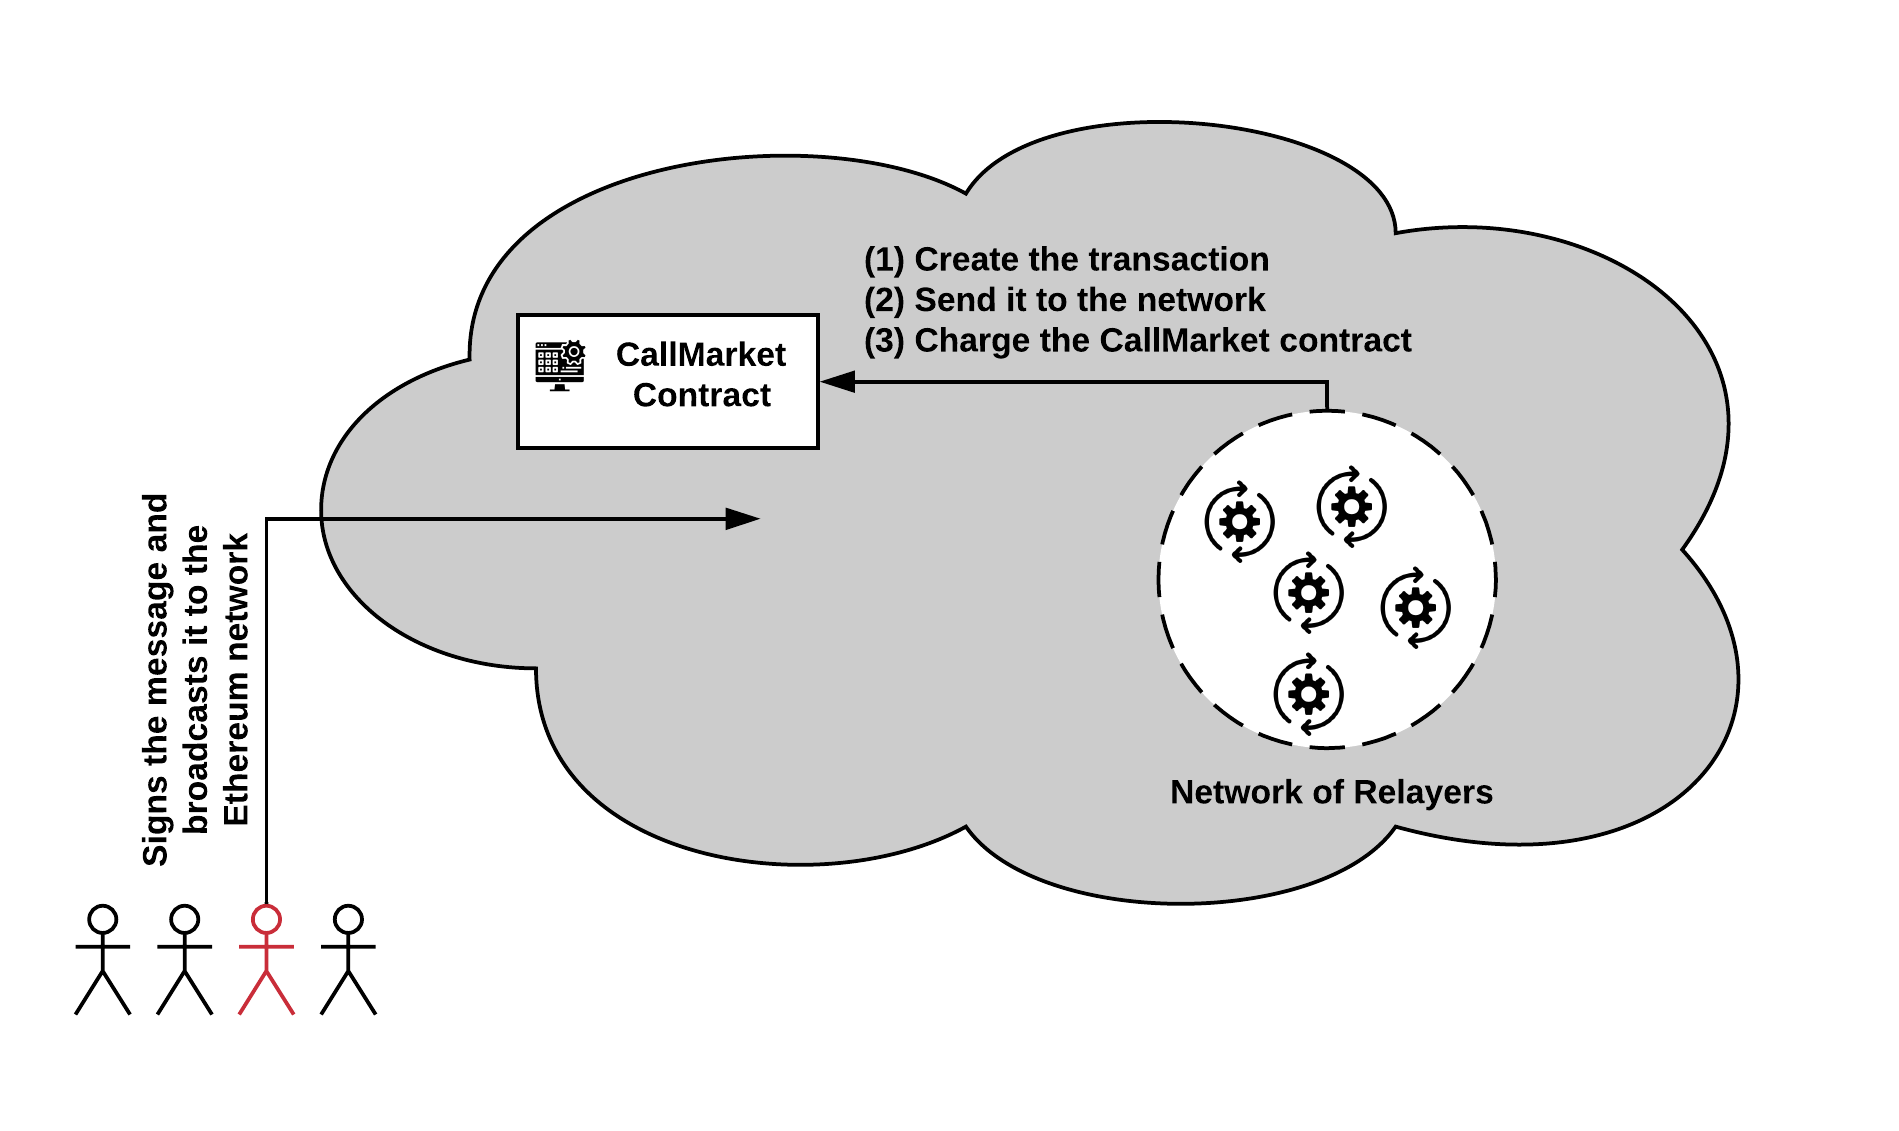
\includegraphics[width=0.8\textwidth]{fig/meta_tx.png}
\caption{\footnotesize{}  \label{fig:meta_tx}}
\end{figure}

% = = = = = = = = = = = = = = = = = = = = = = = = = = = = = = = = = %

%= = = = = =  = =  =  Users close and get refunded with the contract funds (collected as fees during order submissions) =  = = = = = = = = =%

\item \textbf{Using the "Contract Pays" Model.} An alternative solution is to design the market such that the last person to submit an order calls the \texttt{CloseMarket()} function, but in contrast to a normal transaction (where the person initiating the transaction must pay the fee), here the CallMarket contract pays the cost for closing the market and matching the orders respectively. To enforce this design we can use Solidity function modifiers; every time a new order is submitted, a function modifier checks whether (i) the auction period has to end and/or (ii) the maximum number of total orders has reached. If any of these two conditions are met, the \texttt{CloseMarket()} will be called. Again, market participants are charged with certain amounts of fees every time they submit an order, these fees are accumulated in the CallMarket. Once the \texttt{CloseMarket()} is successfully executed and orders are matched, the contract transfers its funds to that person. Note that here the person must still have enough gas to cover the execution of the transaction as the funds will be only transferred after the transaction is fully executed. However, market participants are incentivized to do so as they may receive more ethers than they have spent.

%= = = = = =  = =  =  Rollups=  = = = = = = = = =%

\label{sec:rollups}
\item \textbf{Using Rollups.} Rollup is a scaling method that moves the storage and computation of the smart contracts off-chain while maintaining the transaction data on the main chain as call-data. In this technique, any Ethereum user can act as a validator; they can execute the \texttt{CloseMarket()}function and only post the new state of the contract (the updated balance of traders) in the form of \textit{assertions} to the main chain. Rollups improve scalability, provide faster and cheaper execution of the contracts, and eliminate the gas limit as the contract is no longer executed on-chain.
In the followings we briefly discuss different rollup proposals and techniques. Each approach uses a different method to ensure correction of assertions:


\begin{itemize}

\item \textbf{{Non-interactive Rollups.}} In this rollup technique, assertions are posted together with a validity proof that would be later used by validators to check if the \texttt{CloseMarket()} function has been executed correctly. ZK-Rollup scheme is one of the solutions that uses ZK-SNARKs to prove the validity of the assertions in zero-knowledge. ZK proofs are quick and cheap to verify but they are expensive and time consuming to generate. These proofs could be generated (i) for free or (ii) the CallMarket contract could collect proportional fees for every trade that is successfully executed.

\item \textbf{{Optimistic Rollups.}} In this scheme, assertions are assumed to be valid if there is no dispute posted about them with a certain window of time (a.k.a. "the challenge period'). Here, dispute resolution is a gas-costly method as the CallMarket contract would have to emulate the transaction on-chain to ensure the correctness the assertion. This scheme introduces a tradeoff between privacy and performance as all the assertions are publicly available and accessible. However, here the new state only reflects the updated balances of traders and no secret is involved. 

\item \textbf {{Multi-round Interactive Rollups.}} In this design paradigm, \textit{pending assertions} are posted on-chain and they are open to dispute. Once the challenge period is over and no challenge is submitted, the assertion is confirmed and the CallMarket contract transitions to the new state (\ie updates traders' balances). This scheme takes the overhead for the CallMarket contract to execute the \texttt{Close()} on-chain by using rounds to the dispute resolutions. The two parties (asserter and challenger) must run an interactive protocol and the CallMarket smart contract would have to act as a referee and decides which party's claim is true. Arbitrum is an example of multi-round interactive rollups that uses an efficient challenge-based protocol to penalize the dishonest parties~\cite{kalodner2018arbitrum}. 

\end{itemize}

%= = = = = =  = =  =  SGX=  = = = = = = = = =%

\item \textbf{{Using Trusted Execution Environments.}} Another way of achieving execution of the \texttt{CloseMarket()} function is incorporating the Ethereum blockchain into the Trusted Execution Environments (TEEs) and decoupling the contract execution from consensus mechanism. TEEs enable secure execution of applications in an isolated processing environment called the \textit{enclave}. Here, the enclave could execute the \texttt{CloseMarket()} function off-chain in TEEs and publish an on-chain attestation Quote to the CallMarket contract. The contract then verifies the correctness of the Quote and if validated correctly, it transitions to the new state. Ekiden is an example that uses Intel SGX to solve the scalability and confidentiality issues with the smart contract execution~\cite{cheng2019ekiden}. A drawback of this scheme is in order to achieve confidentiality-preserving smart contracts we have to trust a trusted party in the form of the hardware manufacturer (\eg Intel).


\end{itemize}
% = = = = = = = = = = = = = = = = = = = = = = = = = = = = = = = = = = = = = = = = = = = = = = = = = = = = = = = = = = = = = = = = = = = = =  %
\end{itemize}

% = = = = = = = = = = = =Transferring the Collateral back to the traders = = = = = = = = = = = = =  %
\subsection{Transferring the Collateral back to Traders.}

% Safely returning collateral 
% Options for non-collaterialized markets




% = = = = = = = = = = = = = = = = = = = = = = = = = = = = = = = = = = = = = = = = = = = = = = = = = = = = = = = = = = = = = = = = = = = = =  %



% = = = = = = = = = = = = = = = = = = = = = = = = = = = = = = = = = = = = = = = = = = = = = = = = = = = = = = = = = = = = = = = = = = = = =  %


% = = = = = = = = = = = =Notes Discussed in Meetings = = = = = = = = = = = = =  %

% Our two competitors are Uinswap and Loopring (that uses ZK roll ups):
% 	1- Uniswap: we can argue that in traditional markets we have various traditional exchanges. Each of these exchanges have different trading rules and designs which work for different traders.
%	2- Loopring:
%		2-1: Barrier to entry: In order for a trader to trade specific ERC20 on Loopring, Loopring has to agree to support that token. It might not be difficult and they probably approve the token as long as it is standard compliant.
%		2-2: ZK proofs are quick and cheap to verify but they are expensive and time consuming to generate: (1) now they are generating these proofs for free but later they charge traders for doing that. (2) Looping does not probably generate these proofs per every block so the settlement and 				clearing is not happening per block. So we have faster clearing and settlement as we clear everything per block. 
% 		2-3: Loopring is non-custodial, meaning that the money moves only when the proofs come, so there is a latency in transferring funds to the traders.


% The heap with dynamic array can do 26 pairs of matches at worst case matching whereas Linkedliat does 90 pairs. So if we want to cap the orders over 4 PQs, we’re basically increasing the heap size which makes match more expensive for nothing (every time a match happens and the root is deleted the whole heap is reheapified)

% There will be no ties as we use 2 counters for buy and sell orders. These counters are concatenated them with the price. So we somehow enforce time priority


% = = = = = = = = = = = = = = = = = = = = = = = = = = = = = = = = = = = = = = = = = = = = = = = = = = = = = = = = = = = = = = = = = = = = =  %

% = = = = = = = = = = = = = = = = = = = = = = = = = = = = = = = = = = = = = = = = = = = = = = = = = = = = = = = = = = = = = = = = = = = = =  %
%The tables I changed after estimateGas, Not sure which ones to keep. Should talk to Jeremy 


%
%% = = = = = = = = = = = =Gas costs and refunds for Dequeueing 50 integers from each PQ  = = = = = = = = = = = = =  %
%
%\begin{table}[]
%\centering
%\begin{tabular}{|c|c|c|c|c|}
%\hline
%
%\textbf{\thead{Priority Queue}}    & \textbf{\thead{Net Cost\\in Gas}}      & \textbf{\thead{Total Cost\\in Gas\\(From \texttt{estimateGas})}}      & \textbf{The Difference}    & \textbf{\thead{Gas Refund \\(Manually Calculated)}} \\ \hline
%
%% = = = = = = = = = = = = = = = = = = = = = = = = = = = = = = = = = = = = = = = = = = = = = = = = = = = = = = = = = = = = = = = = = = = = = = %
%	\textbf{\thead{Heap with \\ Dynamic Array}}         				& 2,518,131               & 3,283,480		& 765,349             & 750,000                       \\ \hline
%% = = = = = = = = = = = = = = = = = = = = = = = = = = = = = = = = = = = = = = = = = = = = = = = = = = = = = = = = = = = = = = = = = = = = = = %
%	\textbf{\thead{Heap with \\ Static Array}}           				& 1,385,307                & 2,150,625     	& 765,318             & 750,000                      \\ \hline
%% = = = = = = = = = = = = = = = = = = = = = = = = = = = = = = = = = = = = = = = = = = = = = = = = = = = = = = = = = = = = = = = = = = = = = = %
%	\textbf{\thead{Mapping with \\ keys stored \\ in Heap}} 		& 2,781,684                & 4,316,229       	& 1,534,545           & 1,500,000                     \\ \hline
%% = = = = = = = = = = = = = = = = = = = = = = = = = = = = = = = = = = = = = = = = = = = = = = = = = = = = = = = = = = = = = = = = = = = = = = %
%	\textbf{Linked List}                       							& 557,085               	& 1,772,085      	& 1,215,000           & 1,200,000                      \\ \hline
%% = = = = = = = = = = = = = = = = = = = = = = = = = = = = = = = = = = = = = = = = = = = = = = = = = = = = = = = = = = = = = = = = = = = = = = %
%	\textbf{\thead{Linked List with \\ Mapping}}          				& 731,514              	& 3,731,514       	& 3,000,000     	  &  3,765,000                       \\ \hline
%% = = = = = = = = = = = = = = = = = = = = = = = = = = = = = = = = = = = = = = = = = = = = = = = = = = = = = = = = = = = = = = = = = = = = = = %
%
%\end{tabular}
%\caption{\footnotesize{The gas metrics associated with dequeuing 50 items from five priority queues.}
%\label{tab:PQUnitTests}}
%\end{table}
%% = = = = = = = = = = = = = = = = = = = = = = = = = = = = = = = = = = = = =  %
%
%% = = = = = = = = = = = = = = = = = = = = = = = = = = = = = = = = = = = = =  %
%\begin{table}[]
%\begin{tabular}{|c|c|c|c|c|}
%\hline
%\multirow{2}{*}{Gas Metrics}                        							& \multicolumn{2}{c|}{Linked List}           						& \multicolumn{2}{c|}{Linked List with Mapping}     					\\ \cline{2-5} 
%% = = = = = = = = = = = = = = = = = = = = = = = = = = = = = = = = = = = = = = = = = = = = = = = = = = = = = = = = = = = = = = = = = = = = = =  = = = = = =  = = = = = = = = = = = = = = = =  = = = = = =  = = = = = = %
%                                                                						& with \texttt{SELFDESTRUCT} 		& without \texttt{SELFDESTRUCT}                	& with \texttt{delete} 		& without \texttt{delete}              		\\ \hline                                                                                                                                                                                                                                                          % = = = = = = = = = = = = = = = = = = = = = = = = = = = = = = = = = = = = = = = = = = = = = = = = = = = = = = = = = = = = = = = = = = = = = =  = = = = = =  = = = = = = = = = = = = = = = =  = = = = = =  = = = = = = %
%                   Net Cost in Gas                          					& 557,085                    			& 721,370                     				& 731,514                     	& 334,689                      				\\ \hline
%% = = = = = = = = = = = = = = = = = = = = = = = = = = = = = = = = = = = = = = = = = = = = = = = = = = = = = = = = = = = = = = = = = = = = = =  = = = = = =  = = = = = = = = = = = = = = = =  = = = = = =  = = = = = = %
%\thead{Total Cost in Gas \\ (from \texttt{estimateGas})} 		& 1,772,085                  			& 736,370                  					& 3,731,514                     	& 1,099,689                       				\\ \hline
%% = = = = = = = = = = = = = = = = = = = = = = = = = = = = = = = = = = = = = = = = = = = = = = = = = = = = = = = = = = = = = = = = = = = = = =  = = = = = =  = = = = = = = = = = = = = = = =  = = = = = =  = = = = = = %
%		    The Difference                                             		& 1,215,000                  			& 15,000                      				& 3,000,000                    	& 765,000                       				\\ \hline
%% = = = = = = = = = = = = = = = = = = = = = = = = = = = = = = = = = = = = = = = = = = = = = = = = = = = = = = = = = = = = = = = = = = = = = =  = = = = = =  = = = = = = = = = = = = = = = =  = = = = = =  = = = = = = %
%
%\end{tabular}
%\caption{\footnotesize{}
%\label{tab:LLvsLLMapping}}
%\end{table}
%% = = = = = = = = = = = = = = = = = = = = = = = = = = = = = = = = = = = = =  %




%======================================== %

% = = = = = = = = = = = = = = = = = = = = = = = = = = = = = = = = = = = = = = = = = =

\section{Concluding Remarks}


 
%\subsubsection*{Acknowledgements.} J. Clark thanks ...































